\section*{End-to-end timing analysis of a distributed embedded system}

    The following are the assumptions used in this assignment:

    \begin{itemize}
        \item No offsets
        \item Within a multi-rate chain, the priority of any task is not higher than the priority of its
        predecessor task within the same node
        \item Receving tasks use polling policy to receive messages from the network
        \item Receiving tasks “just miss” the read access of the messages
    \end{itemize}


    Below is the design of the distributed real-time system:

    \begin{figure}[H]
        \centering
        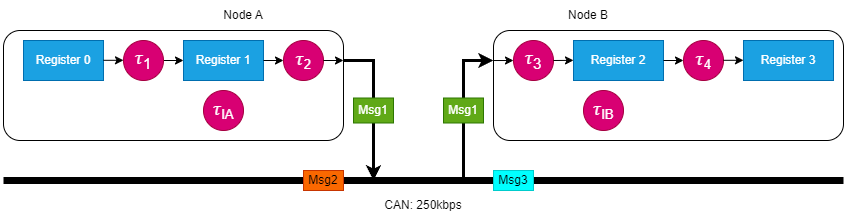
\includegraphics[width=1\textwidth]{images/design.png}
        \caption{Distributed real-time system.}
        \label{fig:design}
    \end{figure}

    The distributed real-time system depicted in figure \ref{fig:design} consists of two nodes, communicating via a CAN-bus with a bit-rate of 250kbps. The nodes each consists of three tasks, two tasks of each node is part of the multi-rate chain which is the transmisttor/receiver of Msg1. The other tasks of each node is meant for some other purpose. However, they can interfere the multi-rate chain and need to be considered in the end-to-end delay analysis. There is a precedence between $\tau_{IA}$ and $\tau_2$, the precedence is defined as $\tau_{IA} < \tau_2$ which means $\tau_2$ cannot execute until $\tau_{IA}$ have finished executing. The specified age and reaction constraint for this chain will be set to $20ms$ and $30ms$ respectively. The tasks in the system have the following parameters:

    \renewcommand{\arraystretch}{1.4}
        \begin{figure}[H]
        \centering
        \begin{minipage}{0.5\textwidth}
            \begin{table}[H]
            \centering
            \begin{tabular}{|l|l|l|l|}
                \hline
                \textbf{Task}   & \textbf{Period = T}   & \textbf{WCET = C} & \textbf{Priority = P} \\ \hline
                $\tau_1$        & 10                    & 1                 & High                  \\ \hline
                $\tau_2$        & 5                     & 1                 & Low                   \\ \hline
                $\tau_3$        & 10                    & 1                 & High                  \\ \hline
                $\tau_4$        & 5                     & 1                 & Low                   \\ \hline
                $\tau_{IA}$     & 2                     & 1                 & Medium                \\ \hline
                $\tau_{IB}$     & 2                     & 1                 & Medium                \\ \hline
            \end{tabular}
            \end{table}
        \end{minipage}
        \caption{Parameters of the tasks in the distributed real-time system.}
        \label{fig:taskparameters}
        \end{figure}
    \renewcommand{\arraystretch}{1.0}

    \subsection*{\textbf{Transmission time of Msg1}}
        The CAN-bus has a bit-rate of 250kbps and the maximum data size of Msg1 is 8 bytes. The transmission of Msg1 is between Node A and Node B via $\tau_1$, CAN-bus and $\tau_2$. The maximum data sizes of Msg2 and Msg3 is set to 8 bytes each. Since they all have the same maximum data size of 8 bytes we will get the same maximum bit size for all messages. The maximum bit size (including stuff bits) is calculated as follows:

        $$maxbitsize = 47+8S_i+\lfloor\frac{34+8S_i-1}{4}\rfloor$$
        
        where $S_i$ is the maximum data size of the message. The maximum bit size of Msg1, Msg2 and Msg3 is calculated as follows:

        $$maxbitsize = 47+(8*8)+\lfloor\frac{34+(8*8)-1}{4}\rfloor = 135 bits$$

        The maximum bit size was calculated using the formula provided in lecture 6. When calculating the transmission time of Msg1, which is needed for the end-to-end delay analysis, the maximum bit size will be used along with the maximum blocking time for Msg1. The maximum blocking time for Msg1 is found by adding the maximum transmission times of Msg2 and Msg3. The maximum transmission times of Msg2 and Msg3 is calculated as follows:

        $$maxtransmissiontime = 47+(8*8)+\lfloor\frac{34+(8*8)-1}{4}\rfloor*\tau_{bit}$$

        where $\tau_{bit}$ is the time to send one bit on the CAN-bus. The $\tau_{bit}$ of the CAN-bus is calculated as follows:

        $$\tau_{bit} = \frac{1}{250000} = 4\mu s$$

        The maximum transmission times of Msg2 and Msg3 is calculated as follows:

        $$maxtransmissiontime = 47+(8*8)+\lfloor\frac{34+(8*8)-1}{4}\rfloor*4 = 540\mu s$$

        To find the maximum blocking time of Msg1 we add the maximum transmission times of Msg2 and Msg3:

        $$maxblockingtime = 540+540 = 1080\mu s$$

        To calculate the worst case transmission time of Msg1 we simply add the $maxblockingtime$ with the maximum transmissiontime of Msg1 (which is the same as for Msg2 and Msg3):

        $$C_{trans} = 1080+540 = 1620\mu s$$

        The worst case transmission time of Msg1 is $1620\mu s$.

    \subsection*{\textbf{Age Dealay and Reaction Delay identified with time line graph (task a)}}
        Below are the time line graphs for the distributed real-time system. The time line graphs are used to identify the age delay and reaction delay of the system. 

        \begin{figure}[H]
            \centering
            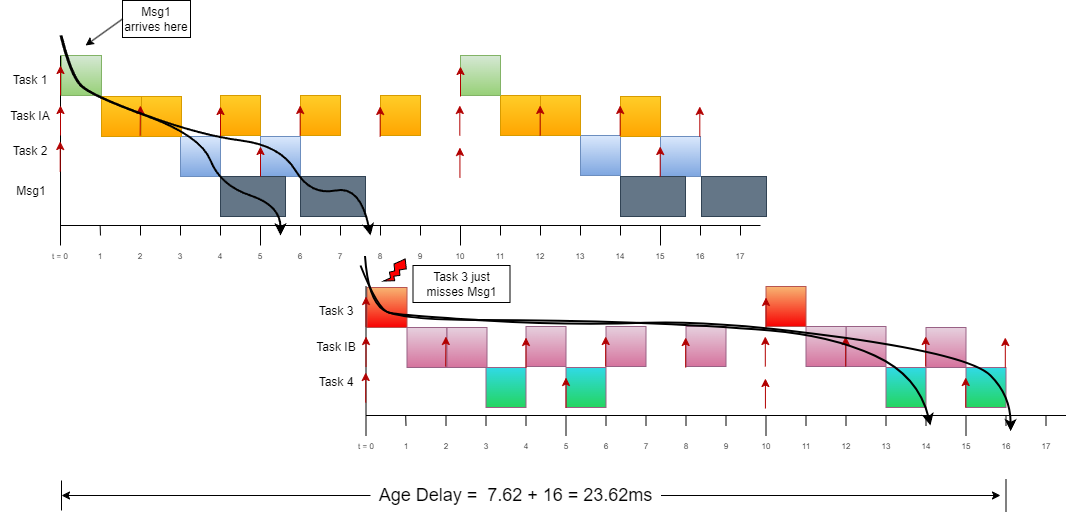
\includegraphics[width=0.8\textwidth]{images/AgeDelay.png}
            \caption{Time line graph for the age delay of the distributed real-time system.}
            \label{fig:agedelay}   
        \end{figure}

        \begin{figure}[H]
            \centering
            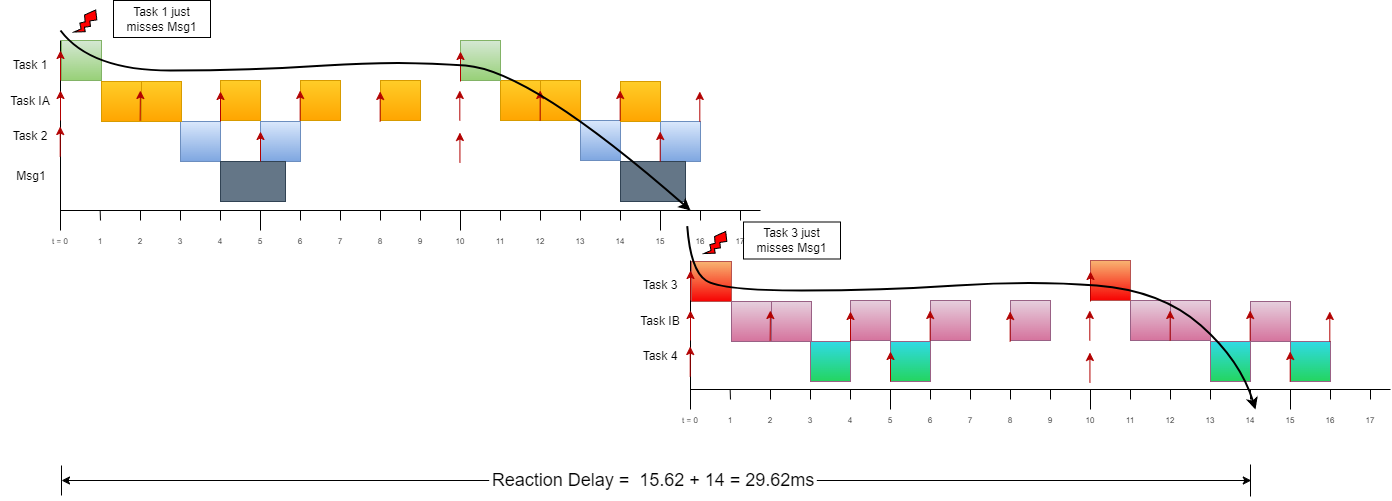
\includegraphics[width=1\textwidth]{images/ReactionDelay.png}
            \caption{Time line graph for the reaction delay of the distributed real-time system.}
            \label{fig:reactiondelay}
        \end{figure}


        \subsection*{Mathematically calculated age delay (task b)}
            The age delay is calculated as follows:

            \textbf{Step 1:} Identiy all reachable timed paths TPs that are initiated in the hyperperiod. 

            \textbf{Step 2:} Calculate the age delay for each TP
            $$Delay = \alpha_{last}(TP^M) + R_{last}(TP^M) - \alpha_{first}(TP^M)$$

            \textbf{Step 3:} Find the maximum age delay among all TPs: 
            $$\text{Age Delay} = max(Delay(TP^1),..,Delay(TP^M))$$

            In the following figure \ref{fig:agedelaypaths}, time paths for age delay is visualized.

            \begin{figure}[H]
                \centering
                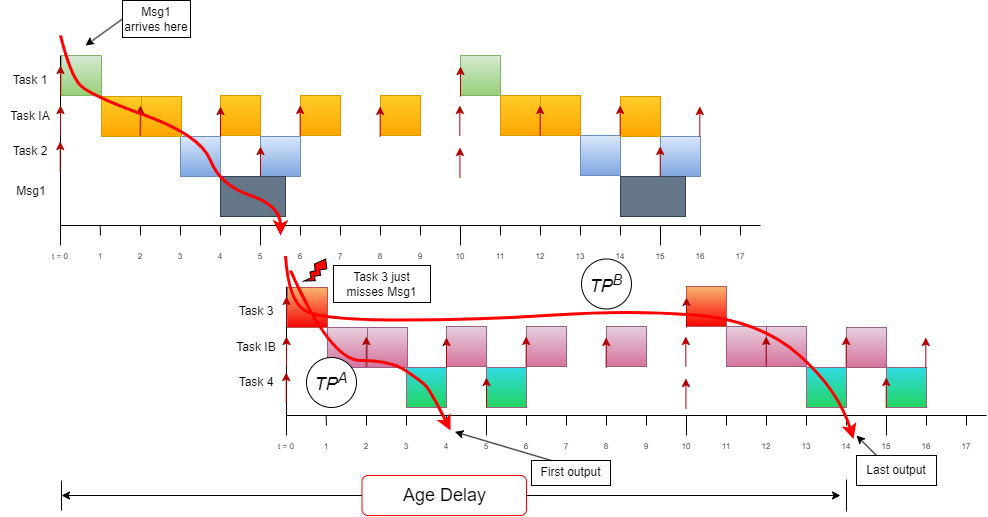
\includegraphics[width=0.8\textwidth]{images/TimedPathAgeDelay.png}
                \caption{Time paths for age delay.}
                \label{fig:agedelaypaths}  
            \end{figure}

            Calculations of the delays are as follows:
            $$Delay(TP^A) = \alpha_4(TP^A) + R_4(TP^A) - \alpha_1(TP^A) = (5.62+3) + 1 - 0 = 9.62ms$$
            $$Delay(TP^B) = \alpha_3(TP^B) + R_3(TP^B) - \alpha_1(TP^B) = (5.62+13) + 1 - 0 = 19.62ms$$
            $$\text{Age Delay} = max(Delay(TP^A), Delay(TP^B)) = 11.62ms$$

            Therefore, the age delay is $19.62ms$.

        \subsection*{\textbf{Mathematically calculated reaction delay (task b)}}
            The reaction delay is calculated using the following steps:

            \textbf{Step 1:} Identify all reachable timed paths in the hyperperiod that have non-duplicate (“first”) output of the chain. Consider the effect of just missing the new data at the input (first task in the chain).

            \textbf{Step 2:} Calculate the delay in each path separately:
            $$Reaction(TP^M) = \alpha_{last}(TP^M) + R_{last}(TP^M) - \alpha_{first}(Pred(TP^M))$$
            where $\alpha_{first}(Pred(TP^M))$ is the activation time of the instance that is predecessor to the instance of the First task
            which is in path $TP^M$.

            \textbf{Step 3:} Find the maximum reaction delay among all TPs: 
            $$\text{Reaction Delay} = max(Reaction(TP^1),..,Reaction(TP^M))$$

            In the following figure \ref{fig:reactiondelaypaths}, time paths for reaction delay is visualized.

            \begin{figure}[H]
                \centering
                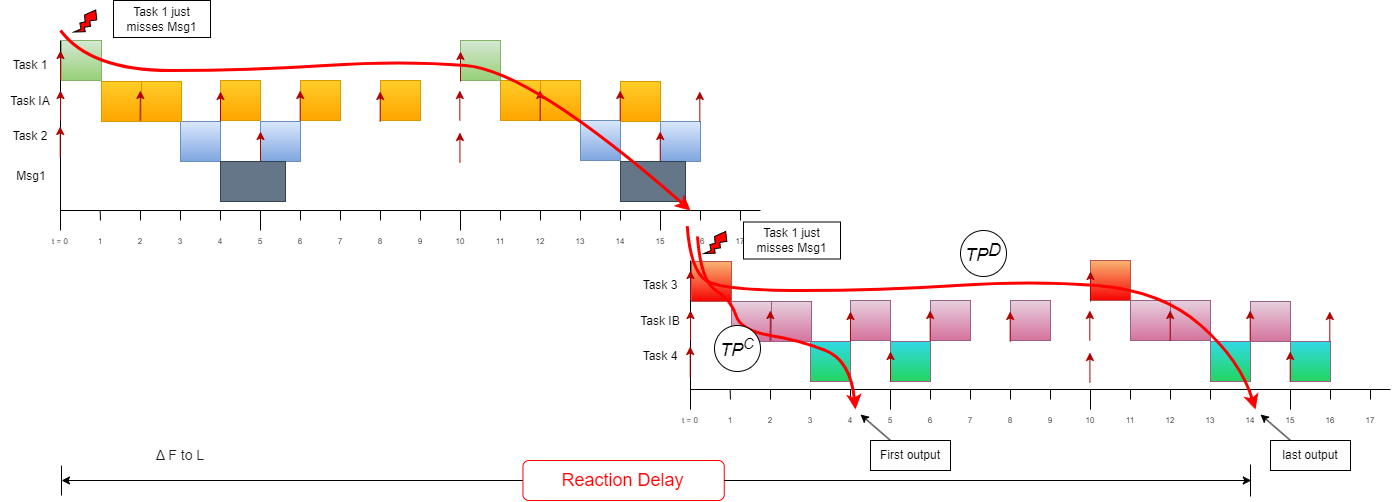
\includegraphics[width=1\textwidth]{images/TimedPathReactionDelay.png}
                \caption{Time paths for reaction delay. In $TP^D$ task 3 just misses the message and therefore has to wait for the next instance of the task execution.}
                \label{fig:reactiondelaypaths} 
            \end{figure}

            Calculations of the delays are as follows: 
            $$Reaction(TP^C) = \alpha_4(TP^C) + R_4(TP^C) - \alpha_{first}(Pred(TP^C)) = (15.62+3) + 1 - 0 = 19.62ms$$
            $$Reaction(TP^D) = \alpha_3(TP^D) + R_3(TP^D) - \alpha_{first}(Pred(TP^D)) = (15.62+13) + 1 - 0 = 29.62ms$$
            $$\text{Reaction Delay} = max(Reaction(TP^C), Reaction(TP^D)) = 29.62ms$$

            Therefore, the reaction delay is $29.62ms$.

        \subsection*{\textbf{Are the specified age and reaction constraints satisfied?}}
            Since the age constraint was set to $20ms$ and the age delay was calculated to $19.62ms$ the age constraint is satisfied. Since the reaction constraint was set to $30ms$ and the reaction delay was calculated to $29.62ms$ the reaction constraint is satisfied. Therefore, both the age and reaction constraints are satisfied.

        \subsection*{\textbf{Consequences of not uing the assumptions given for the assignment}}
            \subsubsection*{No offsets}
                As explained in lecture 6, p.129, the assumption of no offsets is used to simplify the analysis. If the assumption of no offsets was not used, the analysis would be more complex. The assumption is also used to aid in understanding of the end-to-end analysis.

            \subsubsection*{Within a multi-rate chain, the priority of any task is not higher than the priority of its predecessor task within the same node}
                As explained in lecture 6, p.129, the assumption of the priority of any task is not higher than the priority of its predecessor task within the same node is used to simplify the analysis. If the assumption was not used, the analysis would be more complex. The assumption is also used to aid in understanding of the end-to-end analysis.

            \subsubsection*{Receiving tasks use polling policy to receive messages from the network}
                This assumption is used because in a CAN the nodes are not synchronized. Therefore, the receiving tasks need to poll the network to receive the messages. This assumption will also satisfy the assumption of “just missing” the read access of the messages and will make sure we find the worst case reaction delay and age delay.

            \subsubsection*{Receiving tasks “just miss” the read access of the messages}
                Using this assumption will highlight the complexity and issues of using a distributed real-time system. This means that the nodes might be out of synchronization and therefore the receiving tasks might just miss the message. This will result in a higher reaction delay and age delay.
        





  



